\newpage
\section{Teilversuch 2: Bestätigung des Ohmschen Gesetzes}
Fehler bei der Spannungsmessung $\Delta U = \pm 0,5\% \text{ Messwert} + 1 \text{ Digit}$ \\
Fehler bei der Strommessung $\Delta I = \pm 0,8\% \text{ Messwert} + 1 \text{ Digit}$
\begin{equation*}
	\begin{tabu}{l *{10}{l}}
		\toprule
		U/\si{\volt} & 2,07 & 4,08 & 6,01 & 8,02 & 10,06 & 12,15 & 14,14 & 16,09 & 18,02 & 19,99 \\
		\midrule
		I/\si{\milli\ampere} & 0,6 & 1,2 & 1,8 & 2,4 & 3,0 & 3,6 & 4,3 & 4,8 & 5,4 & 6,0 \\
		\bottomrule
	\end{tabu}
\end{equation*}
Die Daten wurden mit \gnuplot{} geplottet und es wurde eine Kurvenanpassung zur $U = mI + c$ durchgeführt. Die entsprechenden Fehler sind im \gnuplot{} direkt berechnet. Für die genaue Rechnung, siehe Appendix \ref{appdx:gnuplottv2}. 
\begin{figure}[H]
	\centering
	% GNUPLOT: LaTeX picture with Postscript
\begingroup
  \makeatletter
  \providecommand\color[2][]{%
    \GenericError{(gnuplot) \space\space\space\@spaces}{%
      Package color not loaded in conjunction with
      terminal option `colourtext'%
    }{See the gnuplot documentation for explanation.%
    }{Either use 'blacktext' in gnuplot or load the package
      color.sty in LaTeX.}%
    \renewcommand\color[2][]{}%
  }%
  \providecommand\includegraphics[2][]{%
    \GenericError{(gnuplot) \space\space\space\@spaces}{%
      Package graphicx or graphics not loaded%
    }{See the gnuplot documentation for explanation.%
    }{The gnuplot epslatex terminal needs graphicx.sty or graphics.sty.}%
    \renewcommand\includegraphics[2][]{}%
  }%
  \providecommand\rotatebox[2]{#2}%
  \@ifundefined{ifGPcolor}{%
    \newif\ifGPcolor
    \GPcolortrue
  }{}%
  \@ifundefined{ifGPblacktext}{%
    \newif\ifGPblacktext
    \GPblacktexttrue
  }{}%
  % define a \g@addto@macro without @ in the name:
  \let\gplgaddtomacro\g@addto@macro
  % define empty templates for all commands taking text:
  \gdef\gplbacktext{}%
  \gdef\gplfronttext{}%
  \makeatother
  \ifGPblacktext
    % no textcolor at all
    \def\colorrgb#1{}%
    \def\colorgray#1{}%
  \else
    % gray or color?
    \ifGPcolor
      \def\colorrgb#1{\color[rgb]{#1}}%
      \def\colorgray#1{\color[gray]{#1}}%
      \expandafter\def\csname LTw\endcsname{\color{white}}%
      \expandafter\def\csname LTb\endcsname{\color{black}}%
      \expandafter\def\csname LTa\endcsname{\color{black}}%
      \expandafter\def\csname LT0\endcsname{\color[rgb]{1,0,0}}%
      \expandafter\def\csname LT1\endcsname{\color[rgb]{0,1,0}}%
      \expandafter\def\csname LT2\endcsname{\color[rgb]{0,0,1}}%
      \expandafter\def\csname LT3\endcsname{\color[rgb]{1,0,1}}%
      \expandafter\def\csname LT4\endcsname{\color[rgb]{0,1,1}}%
      \expandafter\def\csname LT5\endcsname{\color[rgb]{1,1,0}}%
      \expandafter\def\csname LT6\endcsname{\color[rgb]{0,0,0}}%
      \expandafter\def\csname LT7\endcsname{\color[rgb]{1,0.3,0}}%
      \expandafter\def\csname LT8\endcsname{\color[rgb]{0.5,0.5,0.5}}%
    \else
      % gray
      \def\colorrgb#1{\color{black}}%
      \def\colorgray#1{\color[gray]{#1}}%
      \expandafter\def\csname LTw\endcsname{\color{white}}%
      \expandafter\def\csname LTb\endcsname{\color{black}}%
      \expandafter\def\csname LTa\endcsname{\color{black}}%
      \expandafter\def\csname LT0\endcsname{\color{black}}%
      \expandafter\def\csname LT1\endcsname{\color{black}}%
      \expandafter\def\csname LT2\endcsname{\color{black}}%
      \expandafter\def\csname LT3\endcsname{\color{black}}%
      \expandafter\def\csname LT4\endcsname{\color{black}}%
      \expandafter\def\csname LT5\endcsname{\color{black}}%
      \expandafter\def\csname LT6\endcsname{\color{black}}%
      \expandafter\def\csname LT7\endcsname{\color{black}}%
      \expandafter\def\csname LT8\endcsname{\color{black}}%
    \fi
  \fi
    \setlength{\unitlength}{0.0500bp}%
    \ifx\gptboxheight\undefined%
      \newlength{\gptboxheight}%
      \newlength{\gptboxwidth}%
      \newsavebox{\gptboxtext}%
    \fi%
    \setlength{\fboxrule}{0.5pt}%
    \setlength{\fboxsep}{1pt}%
\begin{picture}(8640.00,5760.00)%
    \gplgaddtomacro\gplbacktext{%
      \csname LTb\endcsname%%
      \put(814,704){\makebox(0,0)[r]{\strut{}$-70$}}%
      \put(814,1332){\makebox(0,0)[r]{\strut{}$-60$}}%
      \put(814,1960){\makebox(0,0)[r]{\strut{}$-50$}}%
      \put(814,2588){\makebox(0,0)[r]{\strut{}$-40$}}%
      \put(814,3215){\makebox(0,0)[r]{\strut{}$-30$}}%
      \put(814,3843){\makebox(0,0)[r]{\strut{}$-20$}}%
      \put(814,4471){\makebox(0,0)[r]{\strut{}$-10$}}%
      \put(814,5099){\makebox(0,0)[r]{\strut{}$0$}}%
      \put(946,484){\makebox(0,0){\strut{}$0,1$}}%
      \put(1714,484){\makebox(0,0){\strut{}$0,2$}}%
      \put(2482,484){\makebox(0,0){\strut{}$0,3$}}%
      \put(3250,484){\makebox(0,0){\strut{}$0,4$}}%
      \put(4018,484){\makebox(0,0){\strut{}$0,5$}}%
      \put(4787,484){\makebox(0,0){\strut{}$0,6$}}%
      \put(5555,484){\makebox(0,0){\strut{}$0,7$}}%
      \put(6323,484){\makebox(0,0){\strut{}$0,8$}}%
      \put(7091,484){\makebox(0,0){\strut{}$0,9$}}%
      \put(7859,484){\makebox(0,0){\strut{}$1$}}%
    }%
    \gplgaddtomacro\gplfronttext{%
      \csname LTb\endcsname%%
      \put(209,2901){\rotatebox{-270}{\makebox(0,0){\strut{}Torsionswinkel $\phi$ ($\si{\degree}$)}}}%
      \put(4594,154){\makebox(0,0){\strut{}$\sin(\alpha/\si{\degree})$}}%
      \csname LTb\endcsname%%
      \put(7256,4893){\makebox(0,0)[r]{\strut{}$-64,51852I + -0,14015$}}%
      \csname LTb\endcsname%%
      \put(7256,4607){\makebox(0,0)[r]{\strut{}Messpunkte}}%
      \csname LTb\endcsname%%
      \put(4594,5429){\makebox(0,0){\strut{}Torsionswinkel $\phi$ gegen $\sin(\alpha/\si{\degree})$}}%
    }%
    \gplbacktext
    \put(0,0){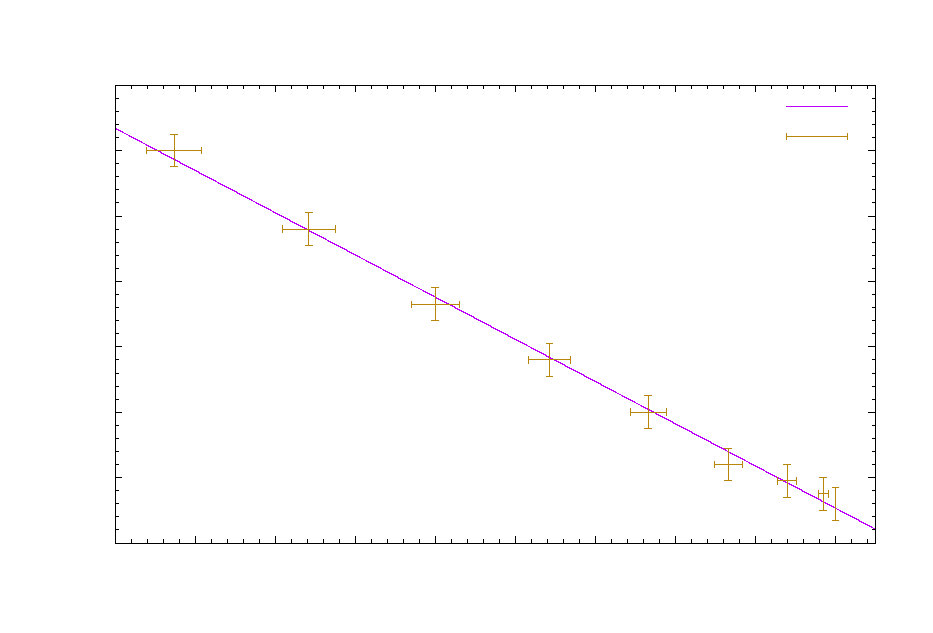
\includegraphics[width={432.00bp},height={288.00bp}]{tv2-plot}}%
    \gplfronttext
  \end{picture}%
\endgroup

	\caption{\centering Bestätigung des Ohmschen Gesetzes \captionbr $\chi^2_{\text{red}} = \num{0.0435856} \implies$ Gute Anpassung}
	\label{fig:tvtwo-plot}
	\vspace{-1em}
\end{figure}
Als Endergebnis erhalten wir:
\begin{equation*}
	\begin{tabu}{lll}
		\toprule
		\text{Variable} & \text{Wert} & \text{Gerundet} \\
		\midrule
		m & \SI{3.3194(161)}{\kilo\ohm} & \SI{3.319(17)}{\kilo\ohm}\\
		c & \SI{0.07578(5424)}{\volt} & \SI{0.08(6)}{\volt} \\
		\bottomrule
	\end{tabu}
\end{equation*}
Aus der Anleitung gilt das Ohmsche Gesetz:
\begin{equation}
	U = I\!R
\end{equation}
Also ist die Steigung den Widerstandwert und es gilt: $R = \SI{3.319(17)}{\kilo\ohm}$. Den Ordinateabschnitt vernachlässigen wir in diesem Fall, weil es sehr klein ist und die Theorie $0$ als Ordinateabschnitt liefert.

Zusammengefasst haben wir:
\begin{center}
	\begin{tabular}{ll}
		\toprule
		Quelle & Widerstandswert \\		
		\midrule
		Hersteller & \SI{3.30(4)}{\kilo\ohm} \\
		Multimeter & \SI{3.290(27)}{\kilo\ohm} \\
		Steigung & \SI{3.319(17)}{\kilo\ohm} \\
		\bottomrule
	\end{tabular}
\end{center}
Das Fehlerintervall aller 3 Widerstandswerten überschneiden sich paarweise miteinander. Die 3 Widerstandswerten stimmen folglich miteinander überein.